\section{Results}


\begin{table}[!htbp] \centering 
  \caption{Characteritics by Sessions} 
  \label{tab:sessions} 
\begin{tabular}{@{\extracolsep{5pt}} cccc} 
\\[-1.8ex]\hline 
\hline \\[-1.8ex] 
Juego & Sesion & No.Participants & Bankrupcy \\ 
\hline \\[-1.8ex] 
PLCS/PLCA & $1$ & $18$ & $0$ \\ 
PLCS/PLCA & $2$ & $15$ & $0$ \\ 
PLCA/PLCS & $1$ & $21$ & $1$ \\ 
PLCA/PLCS & $2$ & $12$ & $0$ \\ 
PL & $1$ & $19$ & $0$ \\ 
PL & $2$ & $18$ & $0$ \\ 
PL & $3$ & $20$ & $0$ \\ 
PH & $1$ & $15$ & $9$ \\ 
PH & $2$ & $20$ & $13$ \\ 
PH & $3$ & $23$ & $16$ \\ 
RL & $1$ & $26$ & $0$ \\ 
RL & $2$ & $16$ & $0$ \\ 
RL & $3$ & $27$ & $2$ \\ 
RH & $1$ & $15$ & $4$ \\ 
RH & $2$ & $15$ & $5$ \\ 
RH & $3$ & $15$ & $6$ \\ 
\hline \\[-1.8ex] 
\end{tabular} 
\end{table} 


A summary of experimental sessions is presented in table \ref{tab:sessions}. All the treatments had three sessions, except for $PLCS$ and $PLCA$ which had only two sessions. In table \ref{tab:rawentry},  we can see the total number of entries in each game by each ideal position. The differences among the number of total trials is due to bankruptcy of the participants that could not longer play.


\begin{table}[!htbp] \centering 
  \caption{Total number of entries by position and game} 
  \label{tab:rawentry} 
\begin{tabular}{@{\extracolsep{5pt}} ccccccc} 
\\[-1.8ex]\hline 
\hline \\[-1.8ex] 
Position & PL & PH & RL & RH & PLCS & PLCA \\ 
\hline \\[-1.8ex] 
Left & 254 &  89 & 254 &  82 & 296 & 299 \\ 
\% & (47) & (23.4) & (39.2) & (23.4) & (89.7) & (90.6) \\ 
Center & 468 & 332 & 630 & 337 & 164 & 263 \\ 
\% & (86.7) & (87.4) & (97.2) & (96.3) & (49.7) & (79.7) \\ 
Right & 468 & 218 & 278 &  82 & 297 & 164 \\ 
\% & (86.7) & (57.4) & (42.9) & (23.4) & (90) & (49.7) \\ 
Total & 540 & 380 & 648 & 350 & 330 & 330 \\ 
\hline \\[-1.8ex] 
\end{tabular} 
\end{table} 


\begin{figure}
	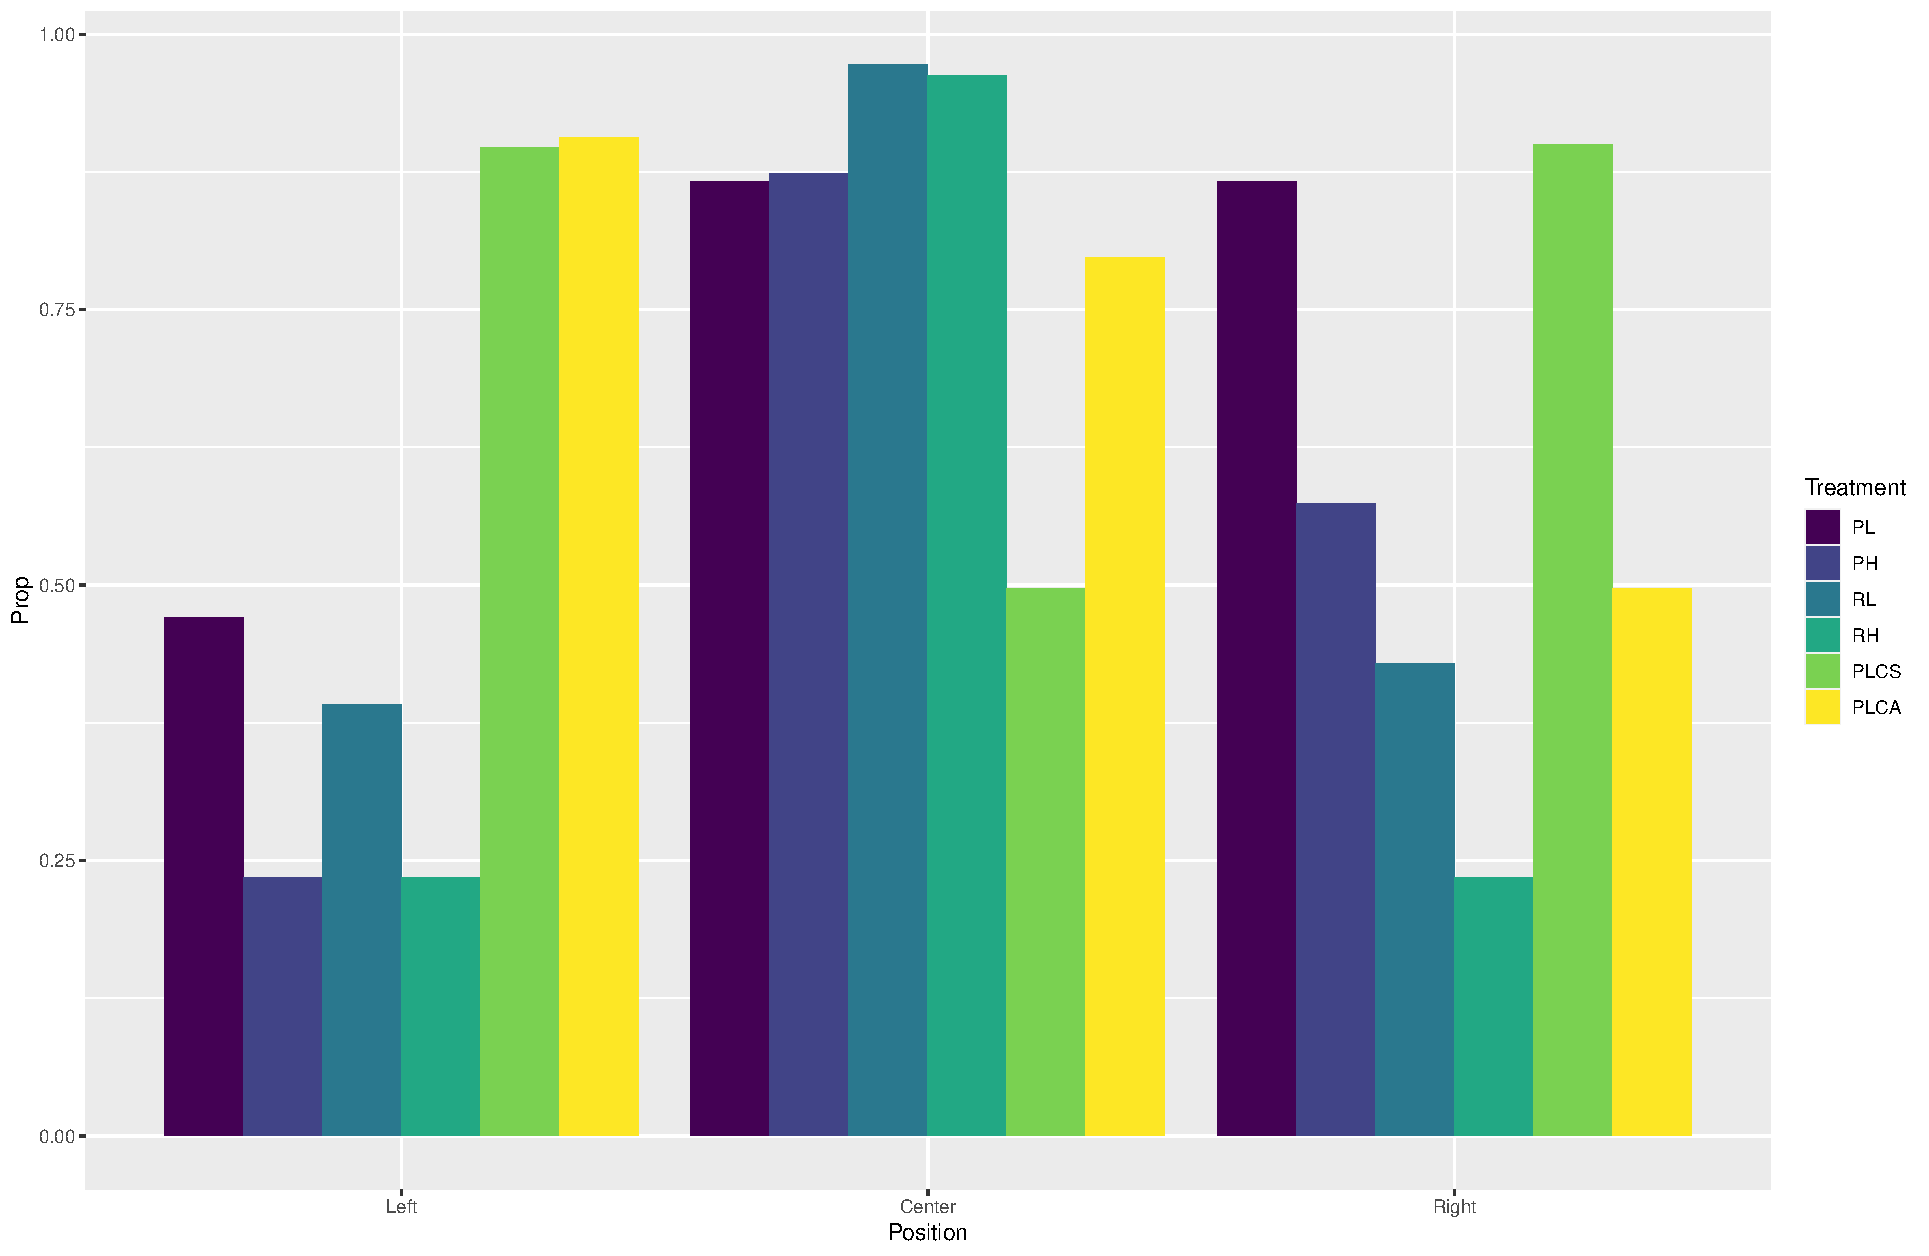
\includegraphics[width=1\linewidth, height=7cm]{../../results/figures/barplot_prop} 
	\caption{Barplot}
	\label{fig:barplot}
\end{figure}

\begin{figure}
	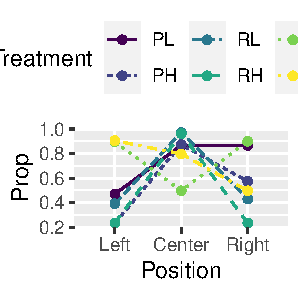
\includegraphics[width=1\linewidth, height=7cm]{../../results/figures/lines_prop} 
	\caption{Lines}
	\label{fig:lines}
\end{figure}


\subsection{Distribution of Errors}

Considering how people behave, it is possible to measure the error as the difference between what participants should have done (choose the option with the highest expected payoff) and what they did (proportion of entry). Then, considering the proportion of entry, a negative value means that they enter less than what is optimal, and a positive value means that they over-participate when they should not. In figure \ref{fig:errordist}, it can be seen the distribution of such error by game and position.


\begin{figure}[h]
	
	\begin{subfigure}{0.5\textwidth}
		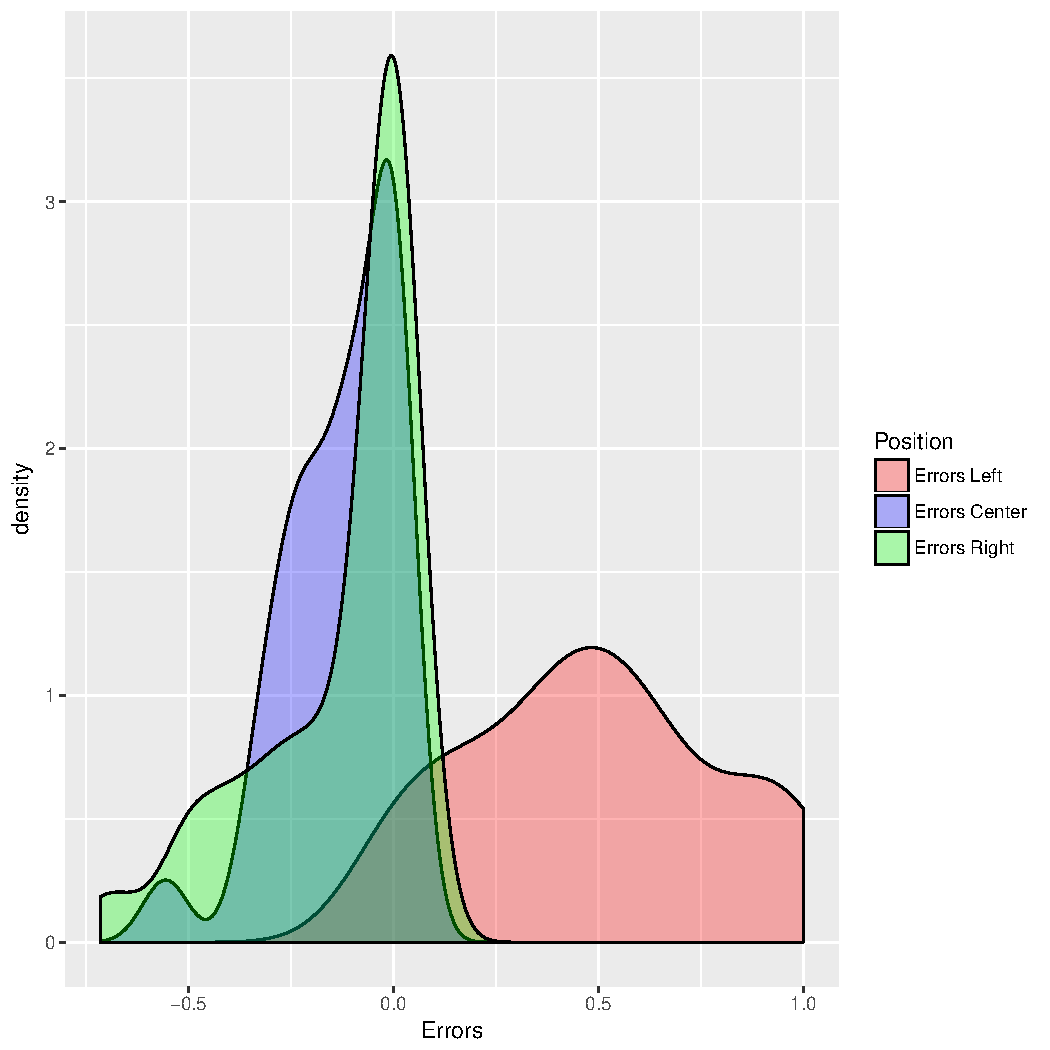
\includegraphics[width=1\linewidth, height=7cm]{../../results/figures/errorDistributionPR_LC} 
		\caption{PR\_LC}
		\label{fig:errdistsubim1}
	\end{subfigure}
	\begin{subfigure}{0.5\textwidth}
		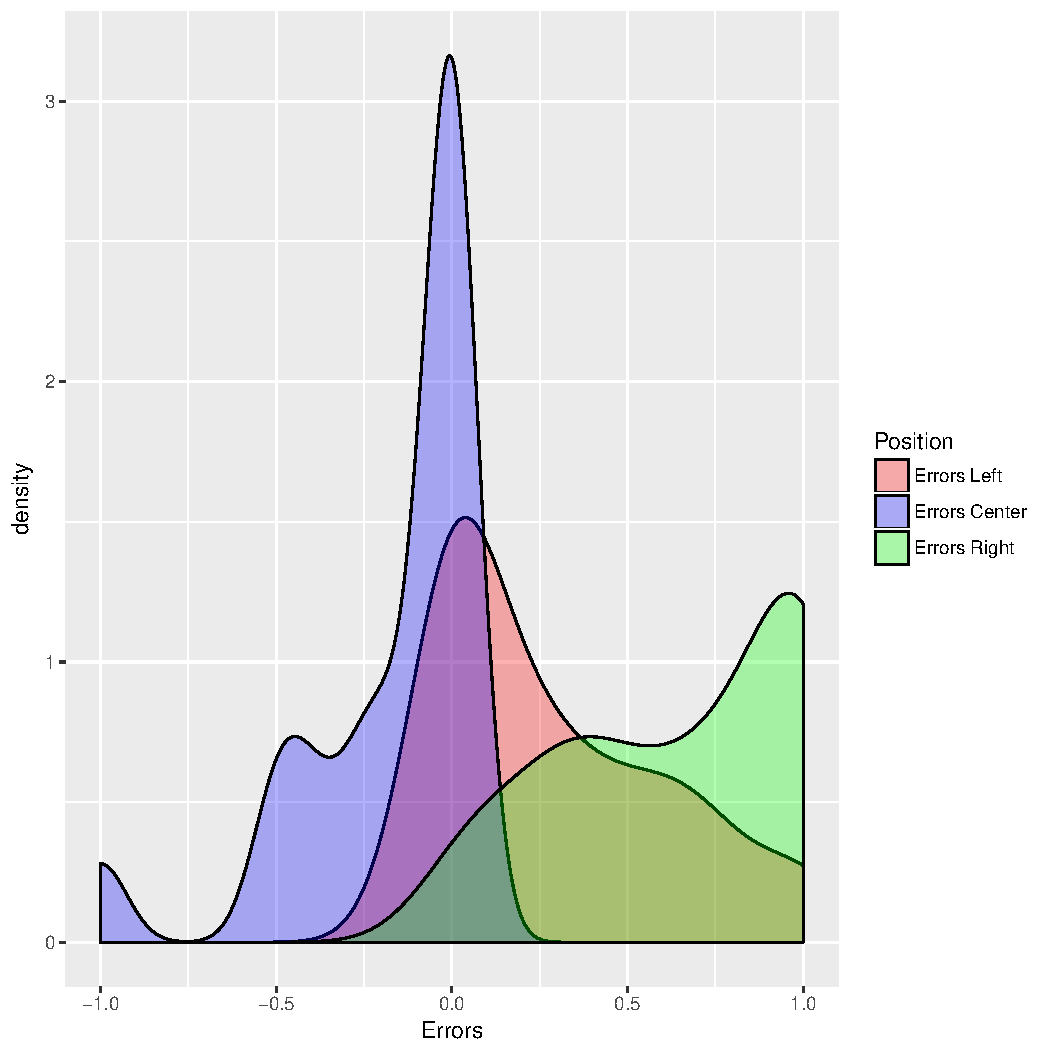
\includegraphics[width=1\linewidth, height=7cm]{../../results/figures/errorDistributionPR_HC}
		\caption{PR\_HC}
		\label{fig:errdistsubim2}
	\end{subfigure}

	\begin{subfigure}{0.5\textwidth}
	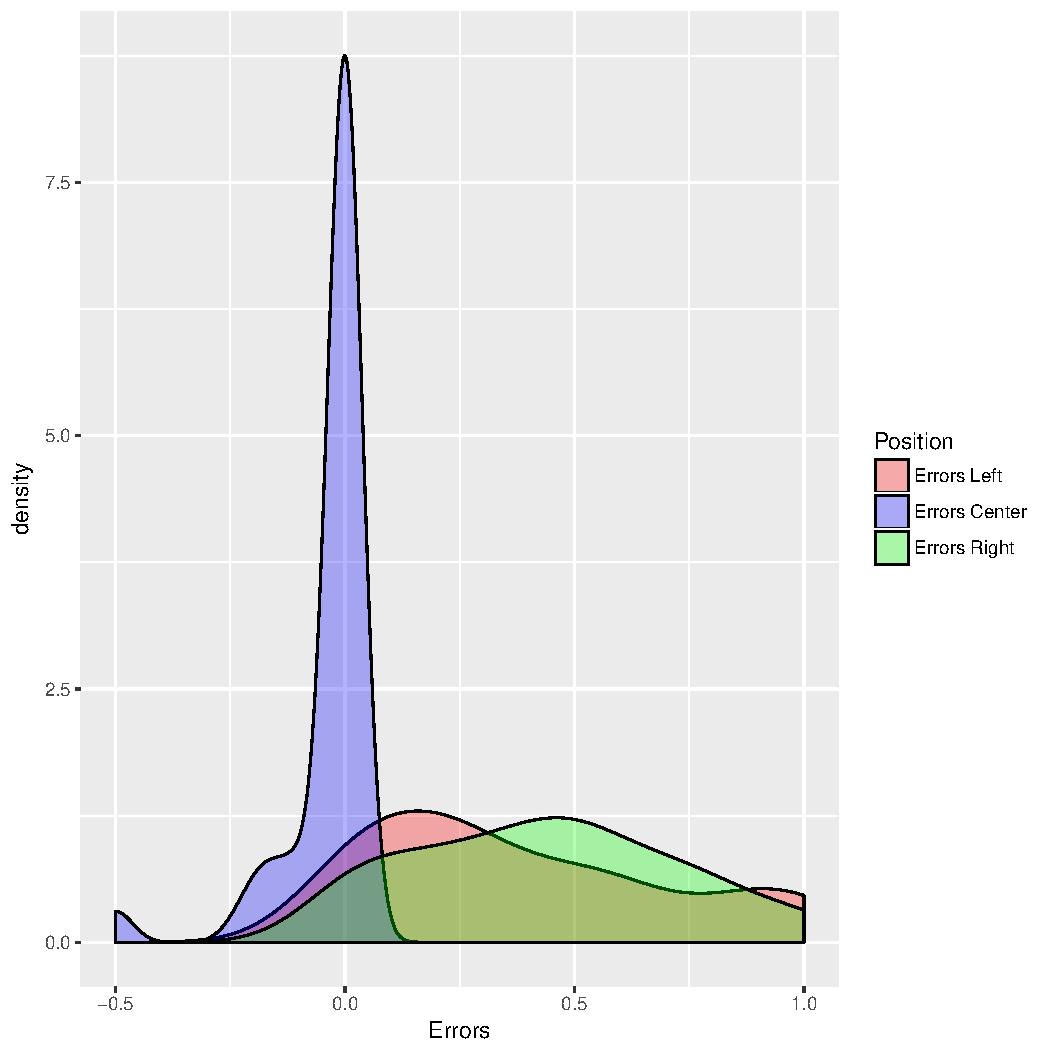
\includegraphics[width=1\linewidth, height=6cm]{../../results/figures/errorDistributionRO_LC} 
	\caption{RO\_LC}
	\label{fig:errdistsubim3}
	\end{subfigure}
	\begin{subfigure}{0.5\textwidth}
	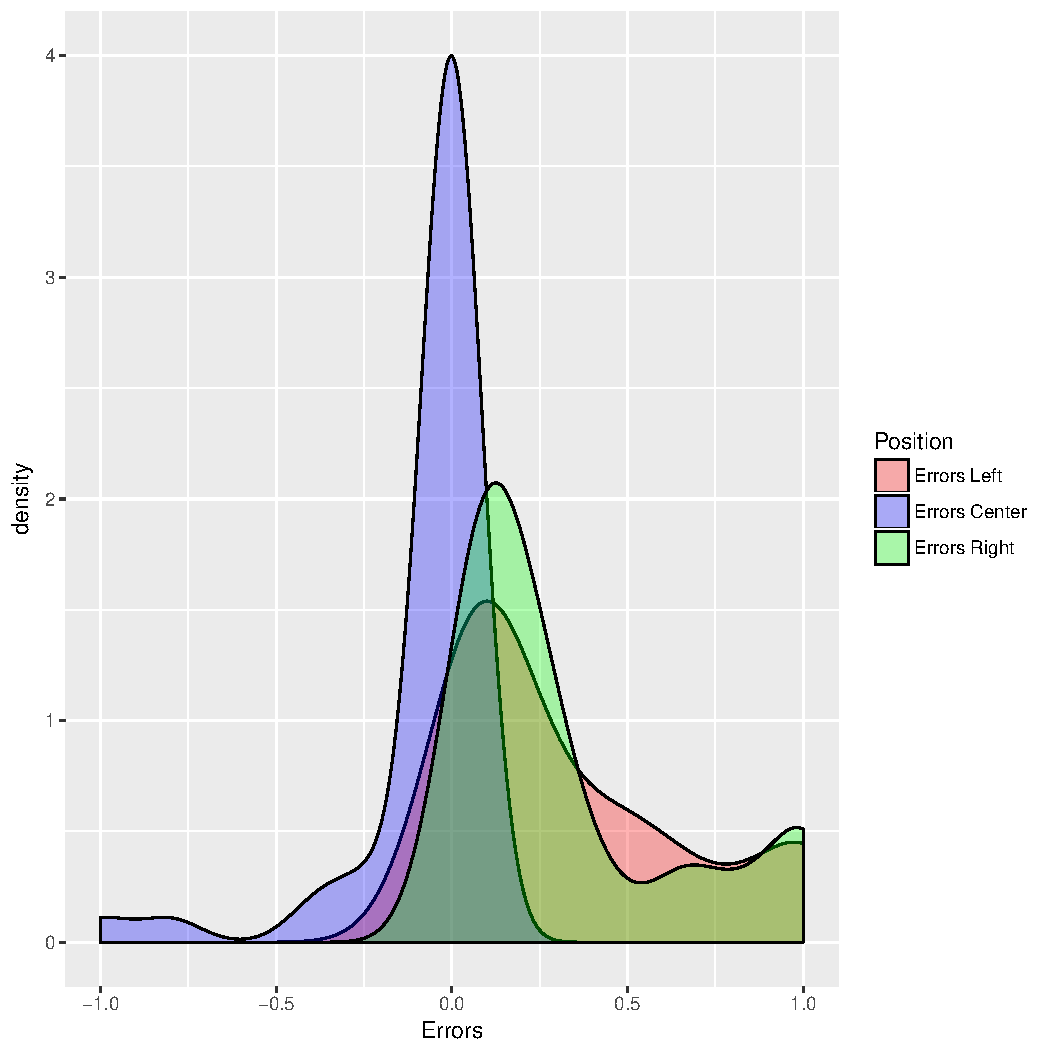
\includegraphics[width=1\linewidth, height=7cm]{../../results/figures/errorDistributionRO_HC}
	\caption{RO\_HC}
	\label{fig:errdistsubim4}
	\end{subfigure}

	\begin{subfigure}{0.5\textwidth}
	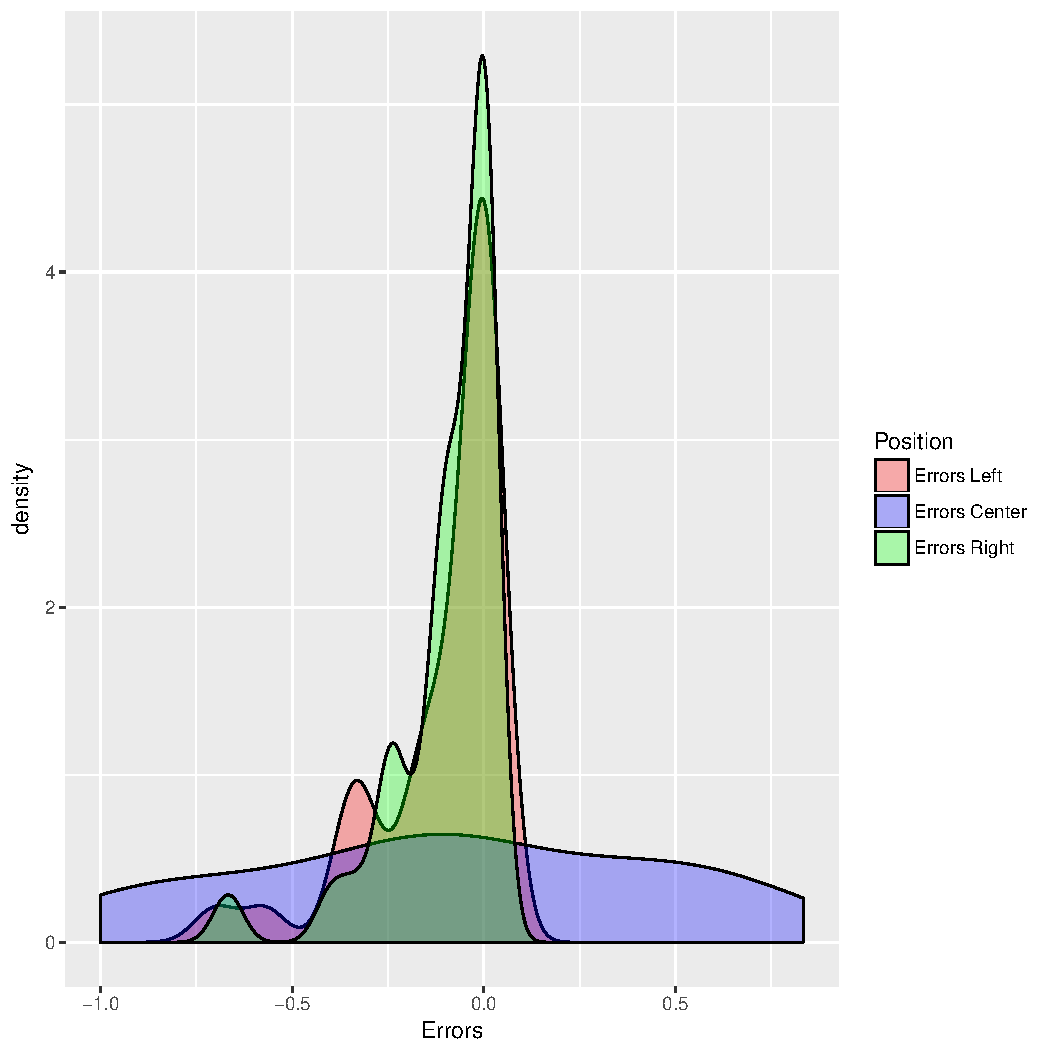
\includegraphics[width=1\linewidth, height=7cm]{../../results/figures/errorDistributionex70} 
	\caption{ex70}
	\label{fig:errdistsubim5}
	\end{subfigure}
	\begin{subfigure}{0.5\textwidth}
	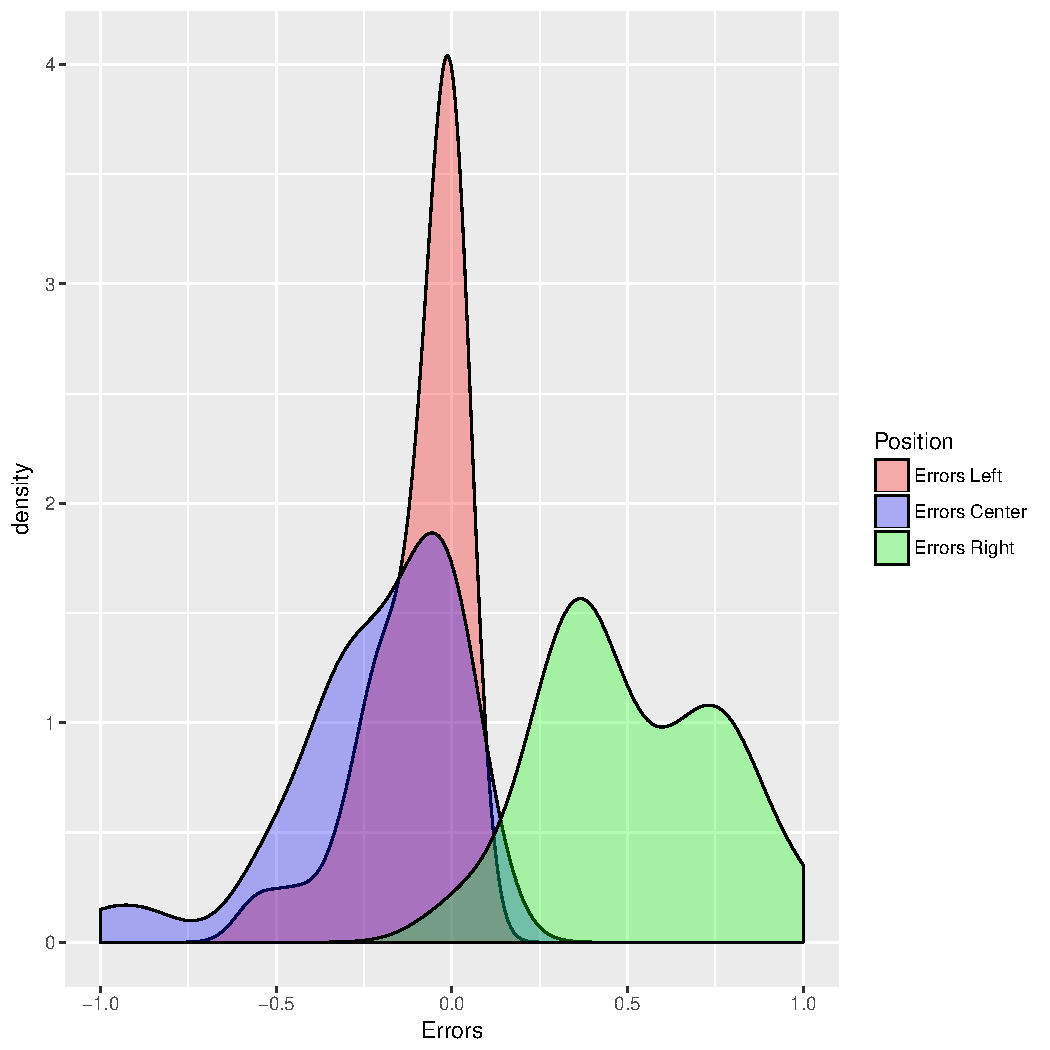
\includegraphics[width=1\linewidth, height=7cm]{../../results/figures/errorDistributionex80}
	\caption{ex80}
	\label{fig:errdistsubim6}
	\end{subfigure}
	
	\caption{Distribution of error by game and position. For each participant, the error was calculated as the difference between the proportion of entry observed and the optimal entry according with the expected payoff calculated based on the entry proportion of all participants in the session.}
	\label{fig:errordist}
\end{figure}


Participants in the central position do not deviate too much from the optimal decision. It is particularly clear in the games whit the same ideal positions $Q=\{20, 30, 80\}$. However, as can be seen in the graph \ref{fig:errdistsubim5}, the behavior in this position is completely random in the game \emph{ex70}, where the extreme positions enter frequently. Furthermore, players in these positions make less mistakes. On the other hand, errors are biased towards over-entering, with some exceptions among participants in the central position. Particularly, in games \emph{PR\_LC} an d\emph{ex80} there is a clear recognition of the over-entering position (figures \ref{fig:errdistsubim1} and \ref{fig:errdistsubim6}). In both cases, that position is the closest to the winning central. This could be due to the fact that, in terms of payoffs, they did not lose too much if the central position wins, but still they continue participating. 

% lets change names

\section{QRE}

The Quantal Response Equilibrium (QRE) proposed by (Richard D McKelvey
and Palfrey 1995) is constructed on the base of a stochastic best
response function. The most used implementation is the logistic function
over the difference between the expected payoff of the options:

\begin{equation}\label{fn:SBR}
\sigma_{ij}= \displaystyle\frac{e^{(\pi_{j})\lambda}}{e^{(\pi_{j})\lambda}+e^{(\pi_{i\ne j})\lambda} } 
=\displaystyle\frac{1}{1+e^{(\pi_{i\ne j}-\pi_{j})\lambda }}        
\end{equation}

The degree of stochasticity in the electionis determined by \(\lambda\). When
\(\lambda \rightarrow 0\) the election is a fair coin tossing for each
option independent of the expected payoffs (minimum level of
rationality), and when \(\lambda \rightarrow \infty\) the election is
deterministic with the more profitable action being chosen with
certainty (complete rationality). The expected payoff of action \(j\) is
represented by \(\pi_j\). Notice that $\pi_j: \sigma_{-i} \rightarrow \mathbb{R}$, where $\sigma_{-i}$ stands for others' distribution of probability.

An easy way to visualize the effect of \(\lambda\) over decisions is to
remember the logistic regression: the dependent variable is the
probability to choose option \(j\), and the independent variable is the
difference between expected payoffs of the two options. Intercept is
fixed in zero -which imply equal probability when options' expected
payoffs are the same-, and slope is precisely \(\lambda\), what
determines how step is the logistic function. For this reason,
\(\lambda\) is also interpreted as the level of rationality: as it
increases, decision will be better in terms of expected payoffs and less
uncertain.


With equation \ref{fn:SBR} a stochastic best response is defined:

\begin{equation}
\sigma^*_{ij}(\lambda, \beta, \pi_{j}(\sigma_{-i}))
\end{equation}\label{eq:SBR} 

, which is the player \(i\)'s probability of choose the
actions \(j\) (i.e.~Entry or Not Entry in the Citizen-Candidate model).
Vector \(\beta\) commonly refers to economic parameters that can measure
risk aversion or altruism. In the present analysis, I do not consider
these possibilities, but because \(\beta\) refers to changes in the
original payoff matrix, I will use \(\beta\) to refer to different
games.

With equation \ref{eq:SBR}, a distribution over actions for each player
is defined: \[\sigma^*_{i}(\lambda, \beta, \sigma_{-i})\]

This stochastic best response have the proprieties of a regular quantal
response function stated by (Goeree, Holt, and Palfrey 2016):

\begin{itemize}
	\item Interiority: $\sigma_{ij} >0$
	\item Continuity: $\sigma_{ij}$ is continuous and differentiable. 
	\item Responsiveness:  $\partial \sigma_{ij} / \partial \pi_{ij} >0 $
	\item Monotonicity: $\pi_{ij}> \pi_{ik} \Rightarrow \sigma_{ij}>\sigma_{ik}$
\end{itemize}

Notice that stochastic best response is a function of others' mixed
strategies (\(\sigma_{-i}\)). This is the case because, as seen in
equation \ref{fn:SBR}, probability depends on \(\pi_{j}\) which is a
function of others' strategies: \(\pi_{j}(\sigma_{-i})\). In the case of
the Citizen-Candidate model, \(\pi_j\) is the expected payoff of
equation \ref{eq:EU}.

Define then the function:

\begin{equation}\label{eq:sigma}
\sigma = (\sigma^*_{1}, ..., \sigma^*_{N})
\end{equation}

Then, quantal response equilibrium (\(\sigma^*\)) is a fixed point of
equation \ref{eq:sigma}, that now is a function only of \(\lambda\) and
\(\beta\). Due to the proprieties of the stochastic best response, and
using the fixed point theorem, the equilibrium existence is assured.
The QRE can be seen as the solution of a non-linear system of equations which is solved numerically. 

Note that a different equilibrium is predicted depending of the value of
\(\lambda\) and that players tend towards pure strategies as \(\lambda\)
goes larger. This equilibrium is called logit equilibrium (Goeree, Holt,
and Palfrey 2016). The software Gambit (Richard D. McKelvey, McLennan,
and Turocy 2014) allows to see those equilibria as a function of the
rationality parameter \(\lambda\). I realized the calculus in \emph{R}
(R Core Team 2017) with the package \emph{nleqslv} (Hasselman 2017), and
compare the result with gambit's; they are the same.

\subsection{Maximul Likelihood Estimation of $\lambda$}

Data analysis at different levels was calculated by maximum likelihood,
following directions from (Goeree, Holt, and Palfrey 2016). The
equilibrium correspondence approach was used: the QRE is calculated for
a given \(\lambda\) and other parameters (\(\beta\)):
\(\sigma*_{ij}(\lambda, \beta)\). In order to find this function, a non
linear equations system with no analytical solution has to be solved.
This was done using the R package \emph{nleqslv} (Hasselman 2017).

Once this function is constructed, it is possible to find the general
logLikelihood objective function, and the then optimize it.

\begin{equation}\label{fn:MLE}
logL(\lambda) = 
\Sigma^n_{i=1} \Sigma^{J_i}_{j=1} f_{i,j} log(\sigma^*_{ij}(\lambda, \beta))
\end{equation}

In the objective function \ref{fn:MLE}: \(n=3\), \(J_i = 2\) and
\(f_{i,j}\) are the times each i-th citizen choose their j-th option. Notice that it was constructed under the assumption of independence of decisions. Also it is assumed that $\lambda$ is the same for all of them.
The Global and by game estimators are in table \ref{tab:mle}.

\begin{table}[!htbp] \centering 
	\caption{} 
	\label{} 
	\begin{tabular}{@{\extracolsep{5pt}} cccccccc} 
		\\[-1.8ex]\hline 
		\hline \\[-1.8ex] 
		X & Global & PR\_LC & PR\_HC & RO\_LC & RO\_HC & ex70 & ex80 \\ 
		\hline \\[-1.8ex] 
		Estimate & $0.078$ & $0.084$ & $0.072$ & $0.098$ & $0.083$ & $0.222$ & $0.075$ \\ 
		sd & $0.001$ & $0.003$ & $0.001$ & $0.004$ & $0.002$ & $0.007$ & $0.004$ \\ 
		\hline \\[-1.8ex] 
	\end{tabular}\label{tab:mle}
\end{table} 

QRE estimation is a punctual number, but the graph of $\sigma (\lambda, \beta)$ can be built for each game. Figure \ref{fig:QRE} displays such function. We can see that when $\lambda=0$ all the players choose entry with $0.5$ probability, and how they approach smoothly towards a some NE. Also, we can see how well the model explain data. Horizontal lines, with their colors corresponding with each player, are the observed proportion in the experiment. Solid vertical line is the global estimate of $\lambda$, and dotted line is the estimation within each game. Where those lines cross is the QRE prediction.

In general, the value of $\lambda$ is similar among games, except for \textit{ex70} game. The estimated is too large compared with the other games, even when it can be seen that prediction is almost perfect. The reasons for this divergence must be investigated more deeply. The worst adjustment is in the \textit{ex80} game where $q_{30}$'s observed proportion of entry is higher than $q_{50}$'s, a fact that QRE cannot explain.

\begin{figure}
	\begin{subfigure}{0.6\textwidth}
		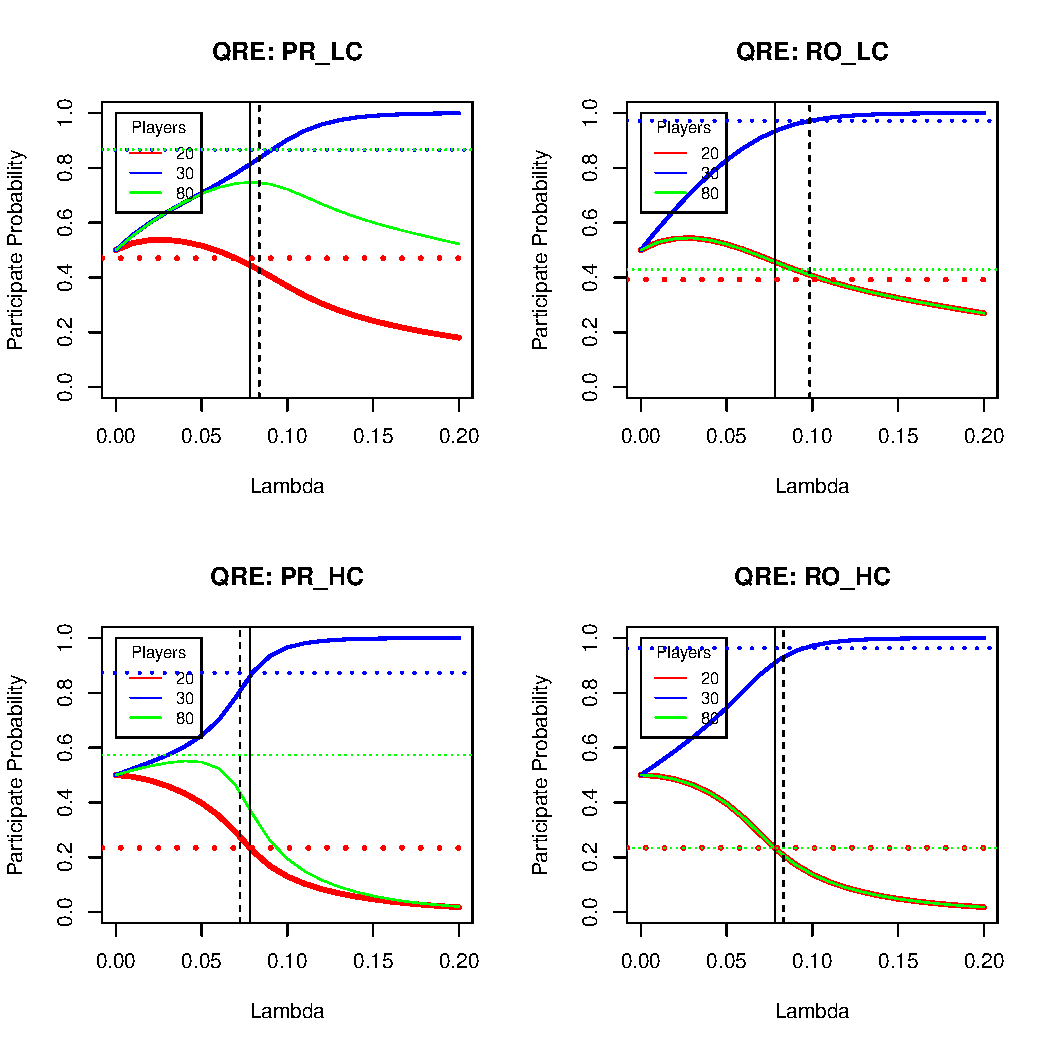
\includegraphics[width=1\linewidth]{../../results/figures/QRE_lambda_MLE}
		\caption{}
		\label{fig:qrelambdamle}
	\end{subfigure}
	\hfill
	\begin{subfigure}{0.7\textwidth}
		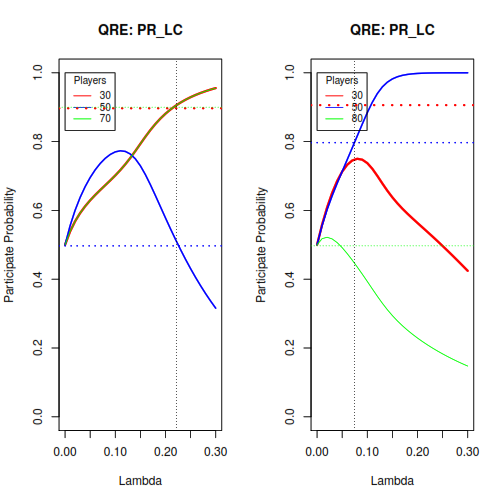
\includegraphics[width=0.6\linewidth]{../../results/figures/1st_treatments_plot}
		\caption{}
		\label{fig:1sttreatmentsplot}
	\end{subfigure}

\caption{QRE expected as a function of $\lambda$}
\label{fig:QRE}
\end{figure}


\subsubsection{Other Equilibria}

Other QRE emerge when $\lambda$ increase if there are other NE because they are especial cases of the QRE when $\lambda\rightarrow\infty$.
When $\lambda$ equals $0$ complete randomness is the only equilibrium, as can be seen in figure \ref{fig:qrelambdamle}. From this point, comes an equilibrium called \emph{logit equilibrium}\cite{Goeree2016}. 
Stochastic best responses seem continuous (even differentiable) functions of the parameter $\lambda$. However, as this parameters increases there will appear other equilibria from anywhere. 

Those equilibria can be seen in figures \ref{fig:ex70eqilibria} and \ref{fig:prlceqilibria}. It is seen as a discrete change in the probability of entry expected for each ideal point. Particularly, in figure \ref{fig:prlceqilibria}, we can see that equilibrium tended towards $q_{30}$ entering alone, and suddenly it is left out the election when $\lambda$ is around $0.15$. On the other hand, in figure \ref{fig:ex70eqilibria}, the contrary pattern is observed when $\lambda$ is around $0.17$.

\begin{figure}[h]
	\begin{subfigure}{0.5\textwidth}
		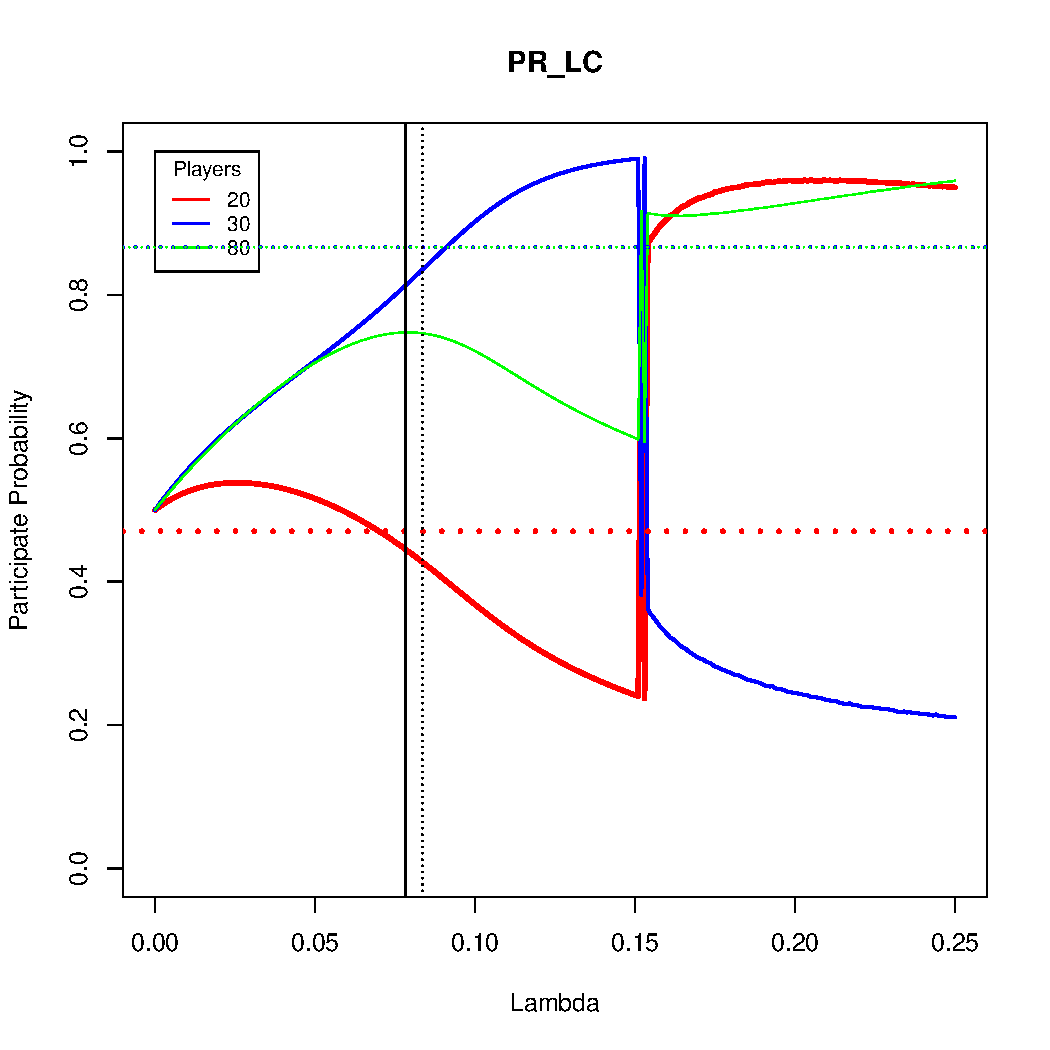
\includegraphics[width=0.7\linewidth]{../../results/figures/PR_LC_eqilibria}
		\caption{}
		\label{fig:prlceqilibria}
	\end{subfigure}
	\hfill
	\begin{subfigure}{0.5\textwidth}
		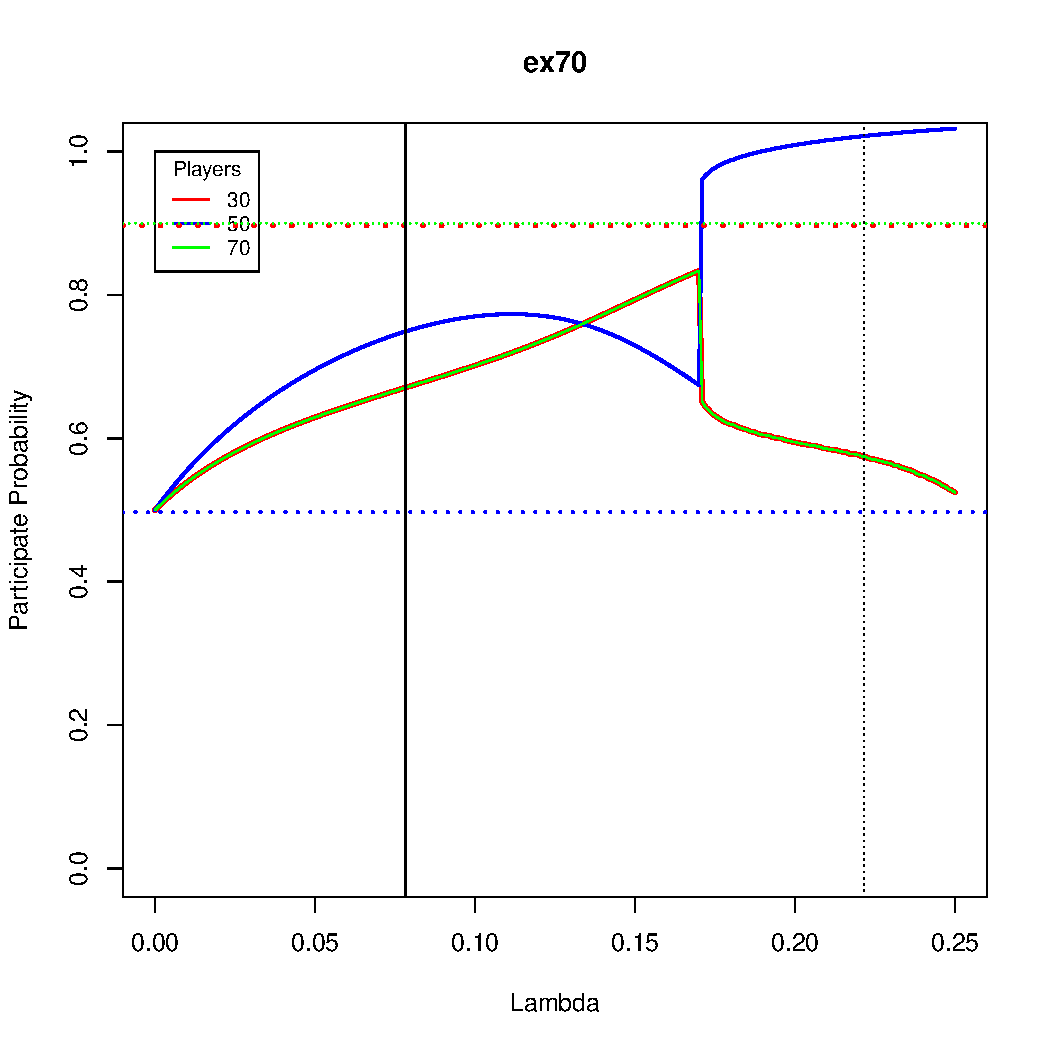
\includegraphics[width=0.7\linewidth]{../../results/figures/ex70_eqilibria}
		\caption{}
		\label{fig:ex70eqilibria}
	\end{subfigure}

\label{fig:otherQRE}
\caption{Other equilibrium that emerge when  $\lambda$ increases.}
\end{figure}
